\documentclass{neu_handout}
\usepackage{url}
\usepackage{amssymb}
\usepackage{amsmath}
\usepackage{marvosym}
\usepackage{graphicx}
\usepackage[pdftex]{graphicx}
\usepackage{subfigure}
\graphicspath{ {images/} }
\everymath{\displaystyle}

% Professor/Course information
\title{Project Proposal: Classification in High-Resolution Brain Scans}
\author{Emily Dutile, Nate Otenti, Asha Chen-Phang, Tristan Sweeney}
\date{April 2018}
\course{EECE}{Pattern Recognition and Machine Learning }

\begin{document}

\section*{1 Abstract}
Being in the multicore and machine learning era, it is important for our machine learning algorithms to take advantage of the potential speed up through the use of paralleling tasks on multicore computers and distributed systems. Using Google's Map Reduce paradigm, we will look to analyze the speed up of a variety of machine learning algorithms for foreground-background classification in high-resolution brain scans. Our project will implement various machine learning algorithms on top of MapReduce to analyze time and processing efficiency.

\section*{2 The Dataset}

We are working with a dataset that comes from scientists who are interested in turning high-resolution brain scans like the one below (left) into a graph representing nerve connections indicated by the bright lines. The original image is 3-dimensional, but for better intuition the 2-dimensional projection on the X-Y plane in shown. As you can see, the image is noisy. However, the axons, which are the lines going across the image, are clearly visible. To
improve the quality of algorithms that automatically trace these axons in an image, we want to classify
each pixel as foreground (belongs to an axon) or background (does not belong to an axon). Intuitively, the traced data looks like the image below (right), where white indicates foreground and black indicates background.\\

\begin{figure}[h]
\centering
{
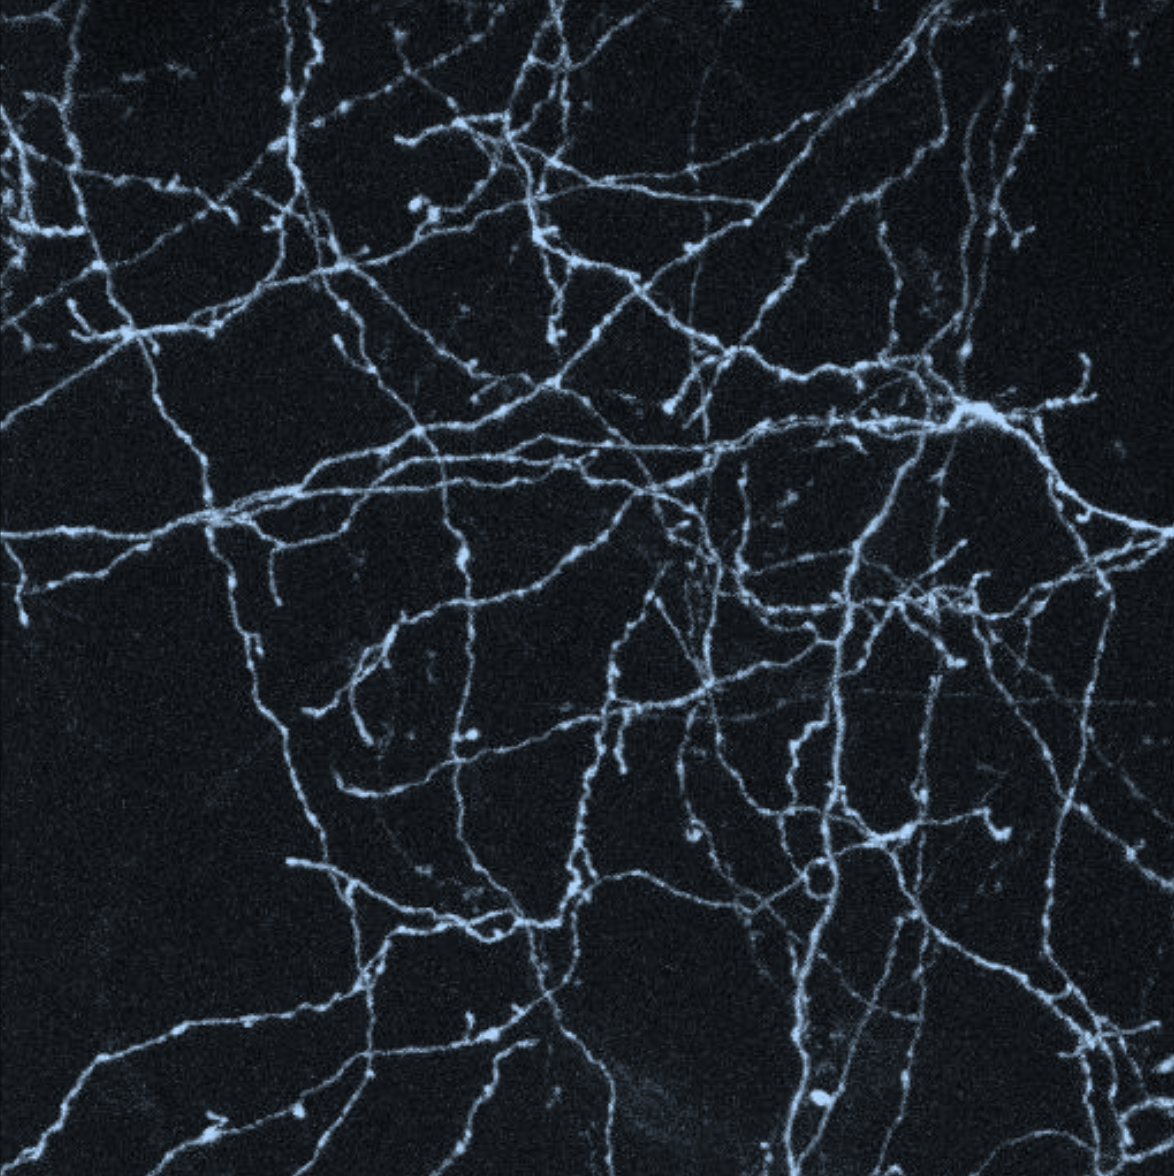
\includegraphics[width=0.2\linewidth]{image1}
}
{
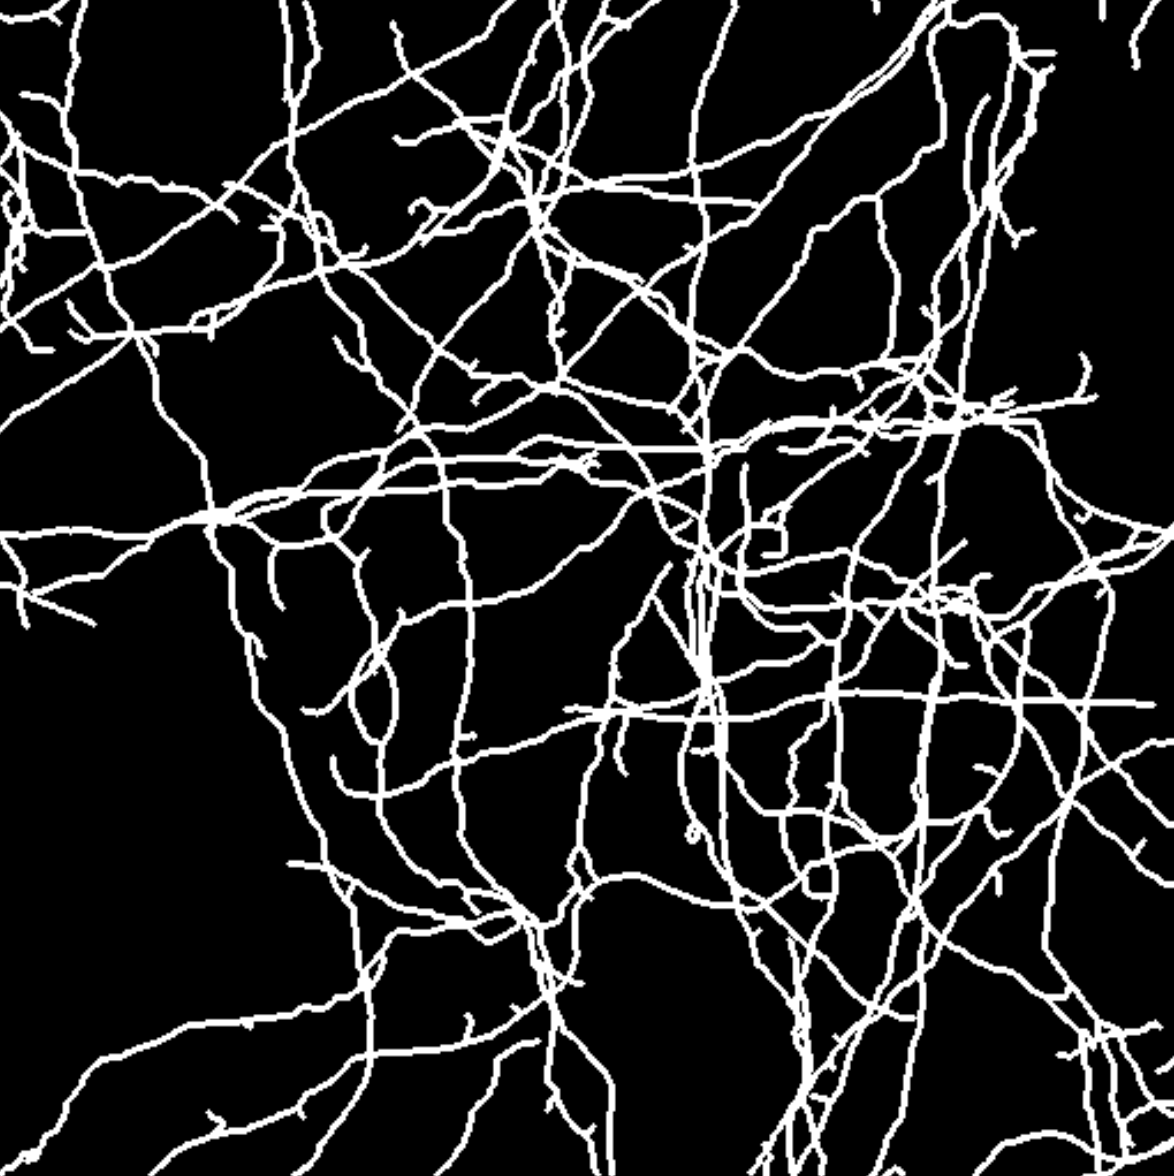
\includegraphics[width=0.2\linewidth]{image2}
}
\end{figure}


Using the manually traced image, the labeled was generated data as follows:

\newenvironment{myitemize}
{ \begin{itemize}
    \setlength{\itemsep}{0pt}
    \setlength{\parskip}{0pt}
    \setlength{\parsep}{0pt}     }
{ \end{itemize}                  } 

\begin{myitemize}
  \item Select a pixel (i, j, k) in the image.
  \item Extract a neighborhood vector centered around (i, j, k).
  \item Extract the label of (i, j, k) from the trace. Here 1 indicates foreground; 0 indicates background.
  \item  Save the record as the neighborhood vector, followed by the label.
\end{myitemize}

Assuming pixel (i=10, j=10, k=10) was selected and we are working with a neighborhood of size 3x3x3, these 27 pixels would be stored as a vector n with 27 elements, where n[0] stores the brightness value of
pixel (9, 9, 9), n[1] the brightness of (9, 9, 10), n[2] of (9, 9, 11), n[3] of (9, 10, 9), n[4] of (9, 10, 10), and so on. Neighborhoods of size 21x21x7 was recommended by domain experts, which is what the labeled data sets contain.\\

The dataset\footnote{\url{https://drive.google.com/drive/u/0/folders/1EJBgJFmp-FQf2czw9LGImoOhEO2OvOoo}} is composed of several labeled csv files, each consisting of rows that contain an input vector of 21x21x7
brightness values (intensity) from a 3D image, together with the center pixel’s foreground-vs-background label. The last value is the label for the whole image. On each line there should be 21*21*7+1 values. The labeled data from images 1, 2, 3, 4, and 6 will be used to train the most accurate model for predicting the labels in image 5 of the datasets.

\section*{3 Prediction Program}
Using Hadoop MapReduce or Spark (Scala), we'll implement a parallel prediction program that uses the previously generated, persisted model to predict for each record in the unlabeled data whether the center pixel is foreground (1) or background (0). Stated differently, this program should replace the “?” label in the unlabeled data by either “0” or “1”, based on the model’s prediction.

\subsection*{3.1 Models}
Using Random Forest, SVM, k-NN and CNN, we will compare how to achieve the best possible accuracy by exploring the parameter combinations. While uniform random partitioning into training and validation data often works well, there are
applications where it is not sufficient, such as this dataset. Assume we have two labeled
records with centers (x, y, z) and (x+1, y+1, z+1), respectively. Uniform sampling might assign (x, y, z) to
training, and (x+1, y+1, z+1) to the validation data. Clearly, the two neighborhoods and the labels of
these two pixels are highly correlated. Hence a model that overfits to the training data will also do very
well on validation pixel (x+1, y+1, z+1). To prevent overly optimistic validation accuracy caused by such
correlations, we have to be more careful when partitioning the labeled data. A safe procedure for 
ensuring independent training and validation data is to partition by image. For example, training data from images 1, 2, 3, and 6; while 4 is used for validation. Alternatively, we can partition each
image into two separate “blocks”, using one block for training data and the other for validation data.\\

Bagging trains each model in an ensemble using bootstrap sampling. All these bootstrap samples have to be taken from the training data. This is the right approach when training data is limited, but in this application, we can produce a training record for each image pixel (minus those too close to the boundary or with unknown labels), then produce even more through rotation and mirroring. Instead of bootstrap samples, we may consider producing a new training set for each model in the ensemble but this may or may not be difficult to achieve in Spark MLlib.

\subsection*{3.2 Evaluation and Testing}
Following the standard way of training and testing a classification model, we will partition the labeled data into 3 separate sets: training data, validation data, and test data. This will be done randomly, such that most data goes into training (60-80\%), and less into the other two (20-10\%). The following steps will be repeated until we are satisfied with the model accuracy: set the model parameters to some values, train the model on the training data using this setting, and then evaluate the model accuracy on the validation data. We can use accuracy (ACC) for the final evaluation. In the final evaluation test set there are about 0.0057 percent foreground and 99.9943 percent background pixels.\\

The output file will be a single file with a single column and as many rows as there are test points. We'll replace all “?” labels with either 1 or 0 and remove all columns except for the label column. All predictions will be stored in plain text.

\section*{4 MapReduce vs. Naive Parallelism}
MapReduce orchestrates distributing work across a distributed system, which naively could be eschewed in favor of directly implementing a multi-node program on a system using a framework such as MPI. Such an approach could be asumed to be more efficent, 'cutting out' the middleman (library) between algorithm and networking. However, when one considers that training a real model on a large corpus of data is a many-hour (or day) process, and during that process machines may experience network failures, system failures, data corruption, etcetera, relying on a framework which provides fault tollerance is well worth the tradeoff (and is easier to work with).

This is not to say that MPI is infeasable for extended time runs, given experienced developers with a defined set of failure cases to be aware of. We certainly don't have the authority to say it shouldn't be used, this is a personal decision by our group to focus on algorithms rather than strict performance.

\begin{thebibliography}{9}
\bibitem{andrewng} 
Map-Reduce for Machine Learning on Multicore,
\\\texttt{http://www.andrewng.org/portfolio/map-reduce-for-machine-learning-on-multicore/}
\end{thebibliography}

\end{document}
